% Author: Alejandro Santomé Valverde

\chapter{Kilo-Scale Programmable Photonics: Design, Integration, and Applications}
\label{chap:systems}

\begin{center}
    \textit{The content of this chapter is largely based on the work accepted for presentation at 
    the 27th European Conference on Integrated Optics (ECIO 2026) \cite{Santome2026_ECIO}. It 
    provides a comprehensive technical extension of the concepts and results reported therein.}
\end{center}
\vspace{1em}

\section{Introduction}

At the core of this chapter lies the objective of maximizing the integration density of 
Programmable Unit Cells to realize truly complex and versatile photonic systems. Commercial and 
academic benchmarks have recently set a high bar for this technology; for instance, the 
\textit{Smartlight} processor by iPronics demonstrates the viability of large-scale integration 
with a programmable hexagonal mesh of 72 PUCs 
\cite{perez-lopezGeneralpurposeProgrammablePhotonic2024a}. Similarly, academic efforts led by Zhang 
and Bogaerts have showcased a general-purpose hexagonal programmable fabric comprising 42 PUCs 
\cite{zhangGeneralPurposeHexagonalProgrammable2026}, further validating the scalability of these 
architectures. 

Rigorous definition of the underlying hardware components is a prerequisite for achieving such 
levels of complexity. In this regard, \cite{gomez-hidalgoFundamentalBuildingBlocks2026} provides a 
comprehensive framework by identifying the fundamental building blocks necessary for scalable 
photonic programmable processors, emphasizing a modular transition from discrete elements to 
interconnected fabrics. However, as noted in recent studies on high-density interconnects for AI 
datacenters \cite{torrijos-moranIndustryInsightPhotonics2026}, scalability is not merely a matter 
of cell count but is fundamentally constrained by signal integrity, cumulative losses, and specific 
application requirements.

Architectural philosophies diverge significantly when addressing these scaling challenges. While 
application-specific designs—such as the feedforward networks optimized for AI workloads and matrix 
multiplication discussed in 
\cite{shenDeepLearningCoherent2017,}—prioritize throughput, they often lack the functional 
flexibility required for general-purpose signal processing. In contrast, the hexagonal 
recirculating meshes presented in this work offer a more versatile alternative 
\cite{perezMultipurposeSiliconPhotonics2017, bogaertsProgrammablePhotonicCircuits2020}. By 
allowing light to circulate through multiple paths and feedback loops, these architectures can 
implement a wider array of functions, ranging from advanced filtering to optical buffering, which 
are unattainable in purely feedforward schemes.

Within large-scale systems, managing the inherent polarization randomness of light coupled from 
standard fibers remains a critical hurdle. To address this, the architecture proposed in this 
chapter adopts a \textbf{polarization diversity} scheme. Utilizing a Polarization Splitter and 
Rotator (PSR), arbitrary input light is separated into its constituent TE and TM components, which 
are then processed independently by dedicated reconfigurable meshes. Such an approach ensures 
robust operation regardless of input conditions and significantly expands the computational 
capacity of the Photonic Integrated Circuit, enabling a higher degree of functional density than 
previously reported.

Representing a major milestone in the field, this chapter introduces a large-scale 
SOI programmable processor featuring 1020 PUCs and 332 integrated photodetectors. Reaching this 
kilo-scale threshold enables the implementation of smart transceiver functions—such as 
dual-polarization routing, fiber interrogation, and dispersion compensation—within a single 
CMOS-compatible chip\cite{Santome2026_ECIO}.



\section{Functional Requirements and Application Framework}
\label{sec:smart_transceiver}

The architecture of this kilo-scale processor represents an evolution in general-purpose programmable 
photonics. While previous application-agnostic designs were often limited to single-polarization 
operation and lacked internal observability—restricting their use to controlled benchtop 
experimentation—the system described here is engineered as an application-ready Silicon-on-Chip 
(SoC). It maintains the inherent flexibility of a programmable hexagonal fabric while satisfying the 
rigorous functional requirements of a software-defined smart transceiver.


Figure \ref{fig:ch4-smart_transceiver} illustrates the integrated signal flow and the specialized 
stages that complement the general-purpose core to enable a truly cognitive optical engine.

\begin{figure}[htbp]
    \centering
    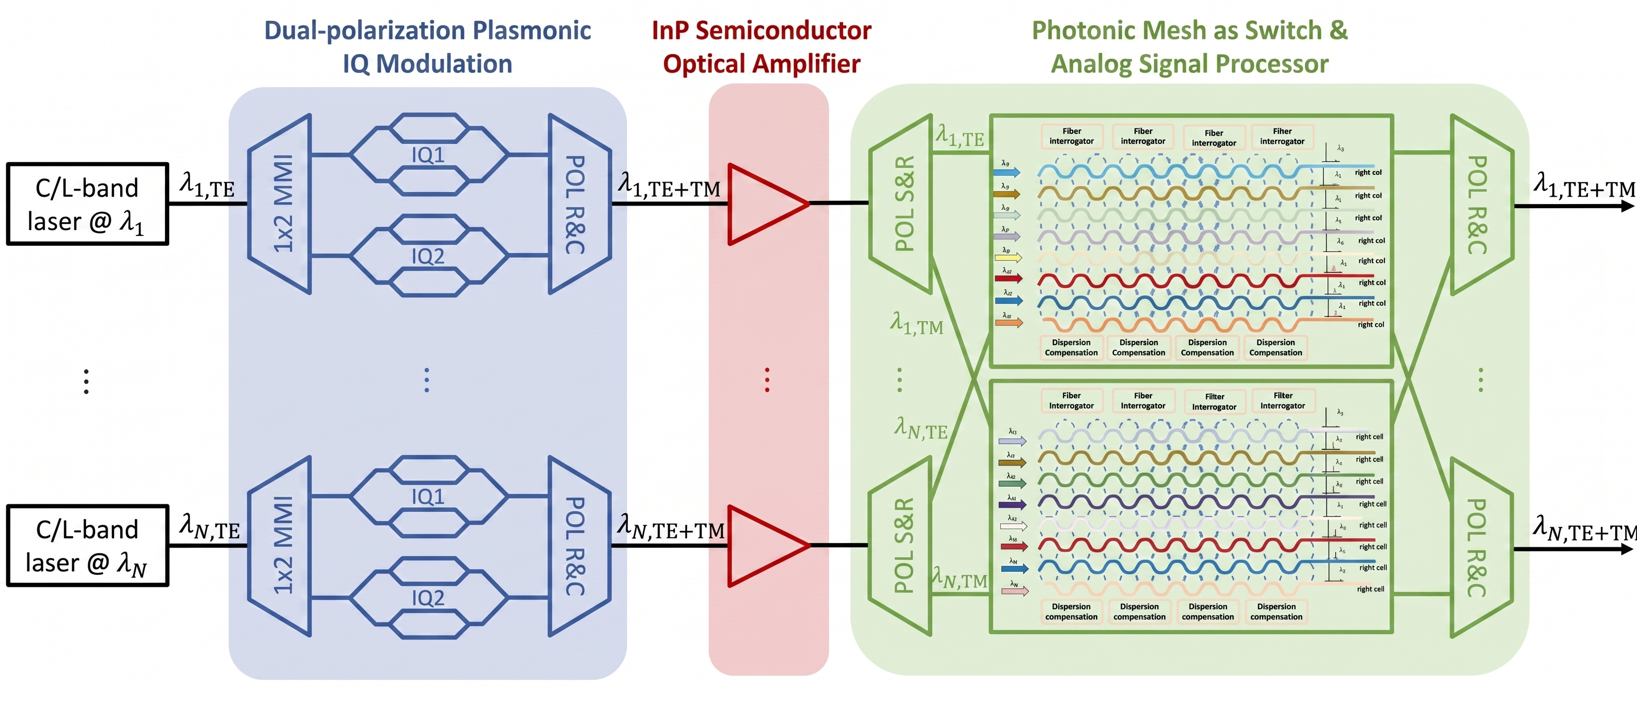
\includegraphics[width=\textwidth]{figures/ch4-smart_transceiver.png} 
    \caption{System architecture of the smart transceiver, highlighting the integration of 
    plasmonic modulation, InP-based amplification, and the reconfigurable dual-polarization SOI 
    core. Schematic courtesy of Dr. Ueli Koch - ETH Zurich \cite{Santome2026_ECIO}.}
    \label{fig:ch4-smart_transceiver}
\end{figure}

To transition from a laboratory prototype to a robust smart transceiver, the PIC must address three 
primary technical pillars:

\begin{enumerate}
    \item \textbf{Full Polarization Transparency and High-Speed Generation:} Unlike standard 
    programmable meshes that require precise input polarization control, this architecture 
    implements a polarization-diversity scheme to process arbitrary fiber-coupled signals. 
    Furthermore, the framework is designed to interface with ultra-high-speed signal generation 
    stages, such as those enabled by plasmonic IQ modulators 
    \cite{smajicPlasmonicElectroOpticModulators2024}. Recent advances in the BTO-on-SiN platform 
    have demonstrated modulation capabilities beyond 200 
    GBd \cite{kohliPlasmonicBTOonSiNPlatform2025}, highlighting the need for a reconfigurable SOI 
    core that can handle such high-capacity data flows across both TE and rotated TM components.

    \item \textbf{Integrated Spectral Interrogation:} To enable real-time link monitoring without 
    external equipment, the chip incorporates two 35-channel Arrayed Waveguide Gratings 
    (AWGs) \cite{Santome2026_ECIO}. These act as on-chip spectrometers, providing high-resolution 
    monitoring for fiber sensing and link characterization \cite{pathakComparisonAWGsEchelle2014}.
    
    \item \textbf{Hybrid Signal Processing:} The design combines the routing flexibility of 1020 PUCs 
    with the high-performance spectral shaping of dedicated lattice filters \cite{Santome2026_ECIO}. This 
    hybrid approach allows the system to mitigate link impairments, such as chromatic dispersion, 
    which are beyond the capabilities of simpler, unassisted general-purpose meshes.
\end{enumerate}

By integrating 332 photodetectors, the processor achieves a level of observability that is critical 
for self-healing and autonomous operation. This massive monitoring layer transforms the 
general-purpose fabric from a passive component into an active, manageable system capable of 
operating in dynamic cognitive optical networks \cite{torrijos-moranIndustryInsightPhotonics2026}.



\section{High-Performance Building Blocks: Design and Characterization}
\label{sec:hpb_design}

To transcend the functional limits of standard programmable meshes, the kilo-scale processor 
integrates specialized High-Performance Building Blocks (HPBs). These components are designed to 
perform complex spectral functions that, while theoretically possible within a universal mesh, would 
require a prohibitive number of Programmable Unit Cells PUCs, leading to excessive insertion losses 
and control complexity. By embedding optimized AWGs and lattice filters, the system achieves a 
hybrid architecture that balances general-purpose flexibility with application-specific performance.

\subsection{Spectral Interrogation: The 35-channel AWG}
\label{subsec:awg_design}

The first pillar of the HPB layer is a pair of Arrayed Waveguide Gratings designed for 
high-resolution spectral monitoring across the C+L bands. Unlike standard AWGs used for simple WDM 
de-multiplexing, these devices are engineered to act as on-chip spectrometers for real-time link 
characterization and fiber sensor interrogation \cite{younOpticalFrequencyMonitoring2001}.

\subsubsection{Design Specifications}

Tailoring the spectral performance of these on-chip spectrometers to the requirements of a smart 
transceiver necessitated a precise definition of their operational parameters. Central to this 
design is the coverage of the full C+L bands, achieved through 35 output channels with a 
standardized channel spacing of 200 GHz ($\sim$1.6 nm). This specific granularity was selected to 
provide a balanced trade-off between the resolution needed for spectral monitoring and the physical 
footprint on the SOI die. To ensure undistorted high-speed signal profiles, the channel bandwidth 
was further optimized in accordance with the requirements for advanced modulation formats 
\cite{chungDemonstrationBidirectionallyTunable2022}.

Governing the spectral response of these spectrometers is the constructive interference condition 
within the device's phased array. For a central wavelength $\lambda_c$, the constant length increment 
between adjacent waveguides in the array, $\Delta L$, must satisfy the fundamental AWG equation:
\begin{equation}
    m \lambda_c = n_{eff} \Delta L
\end{equation}
where $m$ is the diffraction order and $n_{eff}$ represents the effective index of the fundamental 
mode in the array waveguides.

Architectural robustness is further reinforced by the inclusion of 3 input channels, providing the 
redundancy and multi-point interrogation capabilities summarized in Table \ref{tab:awg_specs}. A 
key constraint in this high-density integration was the Free Spectral Range (FSR); at 59.2 nm, the 
FSR acts as a critical guardband to prevent spectral aliasing across the target operational window.
Directly dictated by the path length difference, and accounting for the chromatic dispersion of 
silicon through the group index $n_g$, the FSR is defined as:
\begin{equation}
    FSR = \frac{\lambda_c^2}{n_g \Delta L}
\end{equation}

Precise control over $\Delta L$ thus becomes the primary lever for ensuring that the spectrometer 
covers the C+L bands without ambiguity. Furthermore, the targeted channel spacing 
($\Delta \lambda$) is achieved by adjusting the angular dispersion of the array and the physical 
separation of the output waveguides ($d_o$) at the slab-array interface, following the relation:
\begin{equation}
    \Delta \lambda = \frac{\lambda_c n_s d_o D}{m f n_g}
\end{equation}
where $n_s$ is the refractive index of the slab region, $f$ is the focal length, and $D$ is the 
separation between waveguides in the array.

While telecommunication-grade de-multiplexers typically demand higher isolation, the target 
crosstalk for this system—both inter-channel and intra-channel—was set at -10 dB 
\cite{wangLowlossLowcrosstalk82014}. This threshold is specifically optimized for centroid detection 
algorithms. In the context of fiber sensing, where tracking the relative power distribution is more 
critical than absolute isolation, this level of crosstalk ensures reliable wavelength 
characterization while simplifying the design of the waveguide array and reducing the overall 
insertion loss.

\begin{table}[htbp]
    \centering
    \caption{Target design specifications for the C+L band AWG spectrometer.}
    \label{tab:awg_specs}
    \begin{tabular}{lc}
        \hline
        \textbf{Parameter} & \textbf{Target Value} \\ \hline
        Input Channels & 3 \\
        Output Channels & 35 \\
        Channel Spacing & 200 GHz ($\sim$1.6 nm) \\
        Free Spectral Range (FSR) & 59.2 nm \\
        Inter-channel Crosstalk & $<$ -10 dB \\
        Intra-channel Crosstalk & $<$ -10 dB \\ \hline
    \end{tabular}
\end{table}

\FloatBarrier

\subsubsection{Layout Implementation}

The physical translation of the design targets into a functional SOI layout followed an optimized 
methodology specifically tailored for high-density integration~\footnote{The AWG layout and 
optimization detailed in this section were developed by Dr. J. Fernández.}. This implementation 
phase focused on reconciling the theoretical diffraction order with the physical constraints of the 
220 nm Silicon-on-Insulator platform, utilizing a combination of \textit{EPPiprop} for initial 
synthesis and \textit{FIMMWAVE} for rigorous full-structure verification.

Determining the diffraction order ($m$) constituted the first step of the layout synthesis, 
following the relationship between the central frequency ($f_0$) and the Free Spectral Range: 
$m \approx f_0 / FSR$. To ensure a robust and manufacturable incremental length ($\Delta L$), this 
value was rounded to the nearest integer. Given the specific $\Delta L$ resulting from our target 
FSR, the device was implemented using a Rowland circle geometry with a radius of 200 \textmu m. 
The phased array itself consists of 41 waveguides, an odd number selected to maintain symmetry and 
optimize the field distribution across the array.

Minimizing insertion losses while maintaining low crosstalk required a careful management of the 
waveguide widths and spacings. At the interface with the free propagation regions (FPRs), the 
waveguide width was maximized to 2 \textmu m to capture the maximum possible power, while a gap of 
only 0.2 \textmu m between the 2 \textmu m-wide waveguides in the array was maintained to reduce 
truncation losses. Furthermore, to mitigate the phase errors induced by sidewall roughness—a 
critical factor in SOI waveguides—the array waveguides were transitioned to a larger width in 
their straight sections. 

This design choice, however, necessitated a trade-off with the bending radius. To avoid the 
excitation of higher-order modes in these wider waveguides, a bending radius of 50 \textmu m was 
implemented, coupled with adiabatic transitions to narrower waveguides for the curved sections. 
Finally, the coupling between the array and the input/output waveguides was meticulously simulated 
in \textit{FIMMWAVE} to ensure that the transition to the slab region minimizes reflections and 
losses, thereby securing the -10 dB crosstalk threshold established during the design specification 
phase.

To validate the final layout, rigorous numerical simulations were performed. The resulting spectral 
response, illustrated in Figure \ref{fig:ch4-awg_simulation}, confirms that the device successfully 
achieves the broad spectral coverage required for C+L band operation. The simulation results 
confirm an insertion loss of approximately 6 dB and an FSR of 59.2 nm, evidenced by the spectral 
gaps around 1.52 \textmu m and 1.58 \textmu m. Furthermore, the isolation levels validate the 
design target of -10 dB for both inter-channel and intra-channel crosstalk. 

\begin{figure}[htbp]
    \centering
    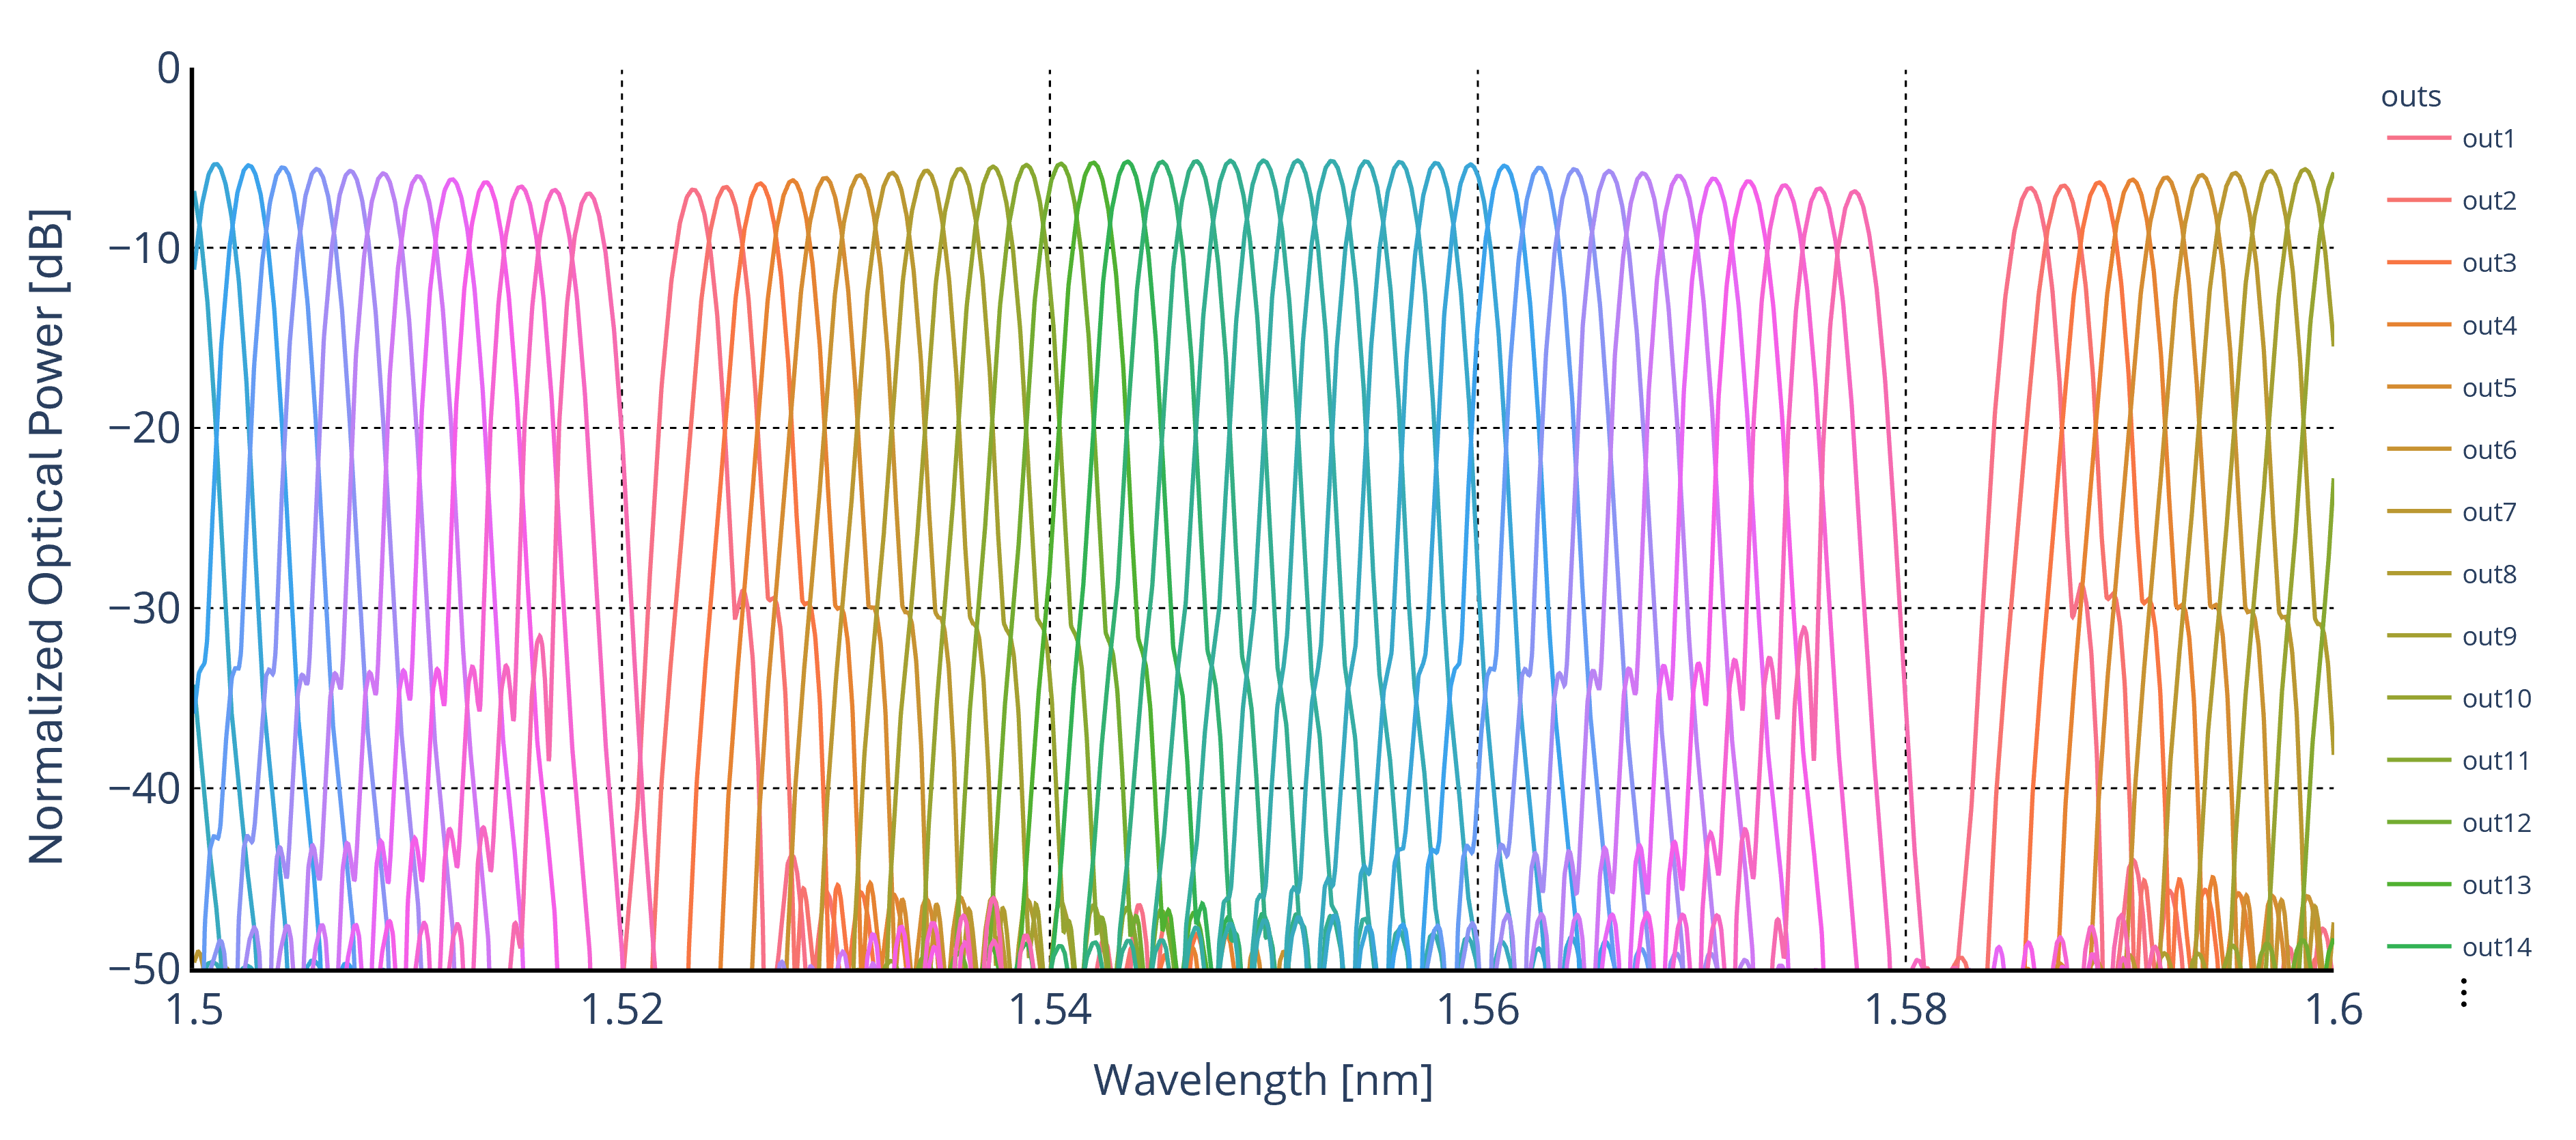
\includegraphics[width=\textwidth]{figures/ch4-awg_simulations.png}
    \caption{Simulated spectral response of the 35-channel AWG spectrometer. The plot illustrates 
    the insertion loss as a function of wavelength, highlighting the periodic nature (FSR) and the 
    achieved crosstalk levels.}
    \label{fig:ch4-awg_simulation}
\end{figure}


\subsubsection{Experimental Characterization}

The performance of the fabricated AWG spectrometers was validated through a dedicated experimental 
characterization phase, conducted upon a serialized test structure included on a specific test PIC. 
To enable accurate fiber-to-chip measurements, the individual input and output ports of the AWG 
were accessed via specialized grating couplers. To account for the spectral dependency of these 
couplers, reference loopback structures were measured in close proximity, allowing for a precise 
de-embedding of the coupling losses from the intrinsic AWG transmission data. Figure 
\ref{fig:ch4-awg_test_structures} details the architecture of this test structure, presenting 
both the GDS layout (a) alongside optical micrographs of the fabricated SOI die (b) and a 
magnification of the free propagation region (c). This components arrangement allows for precise, 
automated spectral scans by moving the input fiber between input ports and sequentially measuring 
the serialized outputs.

Utilizing this specialized setup, characterization involved a tunable C+L band laser source 
and a high-fidelity optical power meter. The PIC was temperature-stabilized at 25~$^\circ$C using a 
Peltier-based TEC to prevent thermo-optic shifts, while the laser was swept with a 0.1~nm resolution 
across the target wavelength range. Resulting normalized transmission spectra for the 35 monitored
output channels are presented in Figure \ref{fig:ch4-awg_measured_spectrum}.

Analysis of the experimental results reveals that the normalized measured insertion loss—which 
accounts for the removal of the grating coupler response—is remarkably low, with most of the values 
below the expected 6dB extracted from simulation. Crucially, the measured crosstalk levels are 
typically around -11~dB, remaining consistent with the -10~dB target threshold required for robust 
centroid detection algorithms. While fabrication tolerances introduce slight variations, the data 
exhibits smooth and well-defined spectral peaks, validating the complex Rowland circle geometry and 
the waveguide array design.

\begin{figure}[htbp]
    \centering
    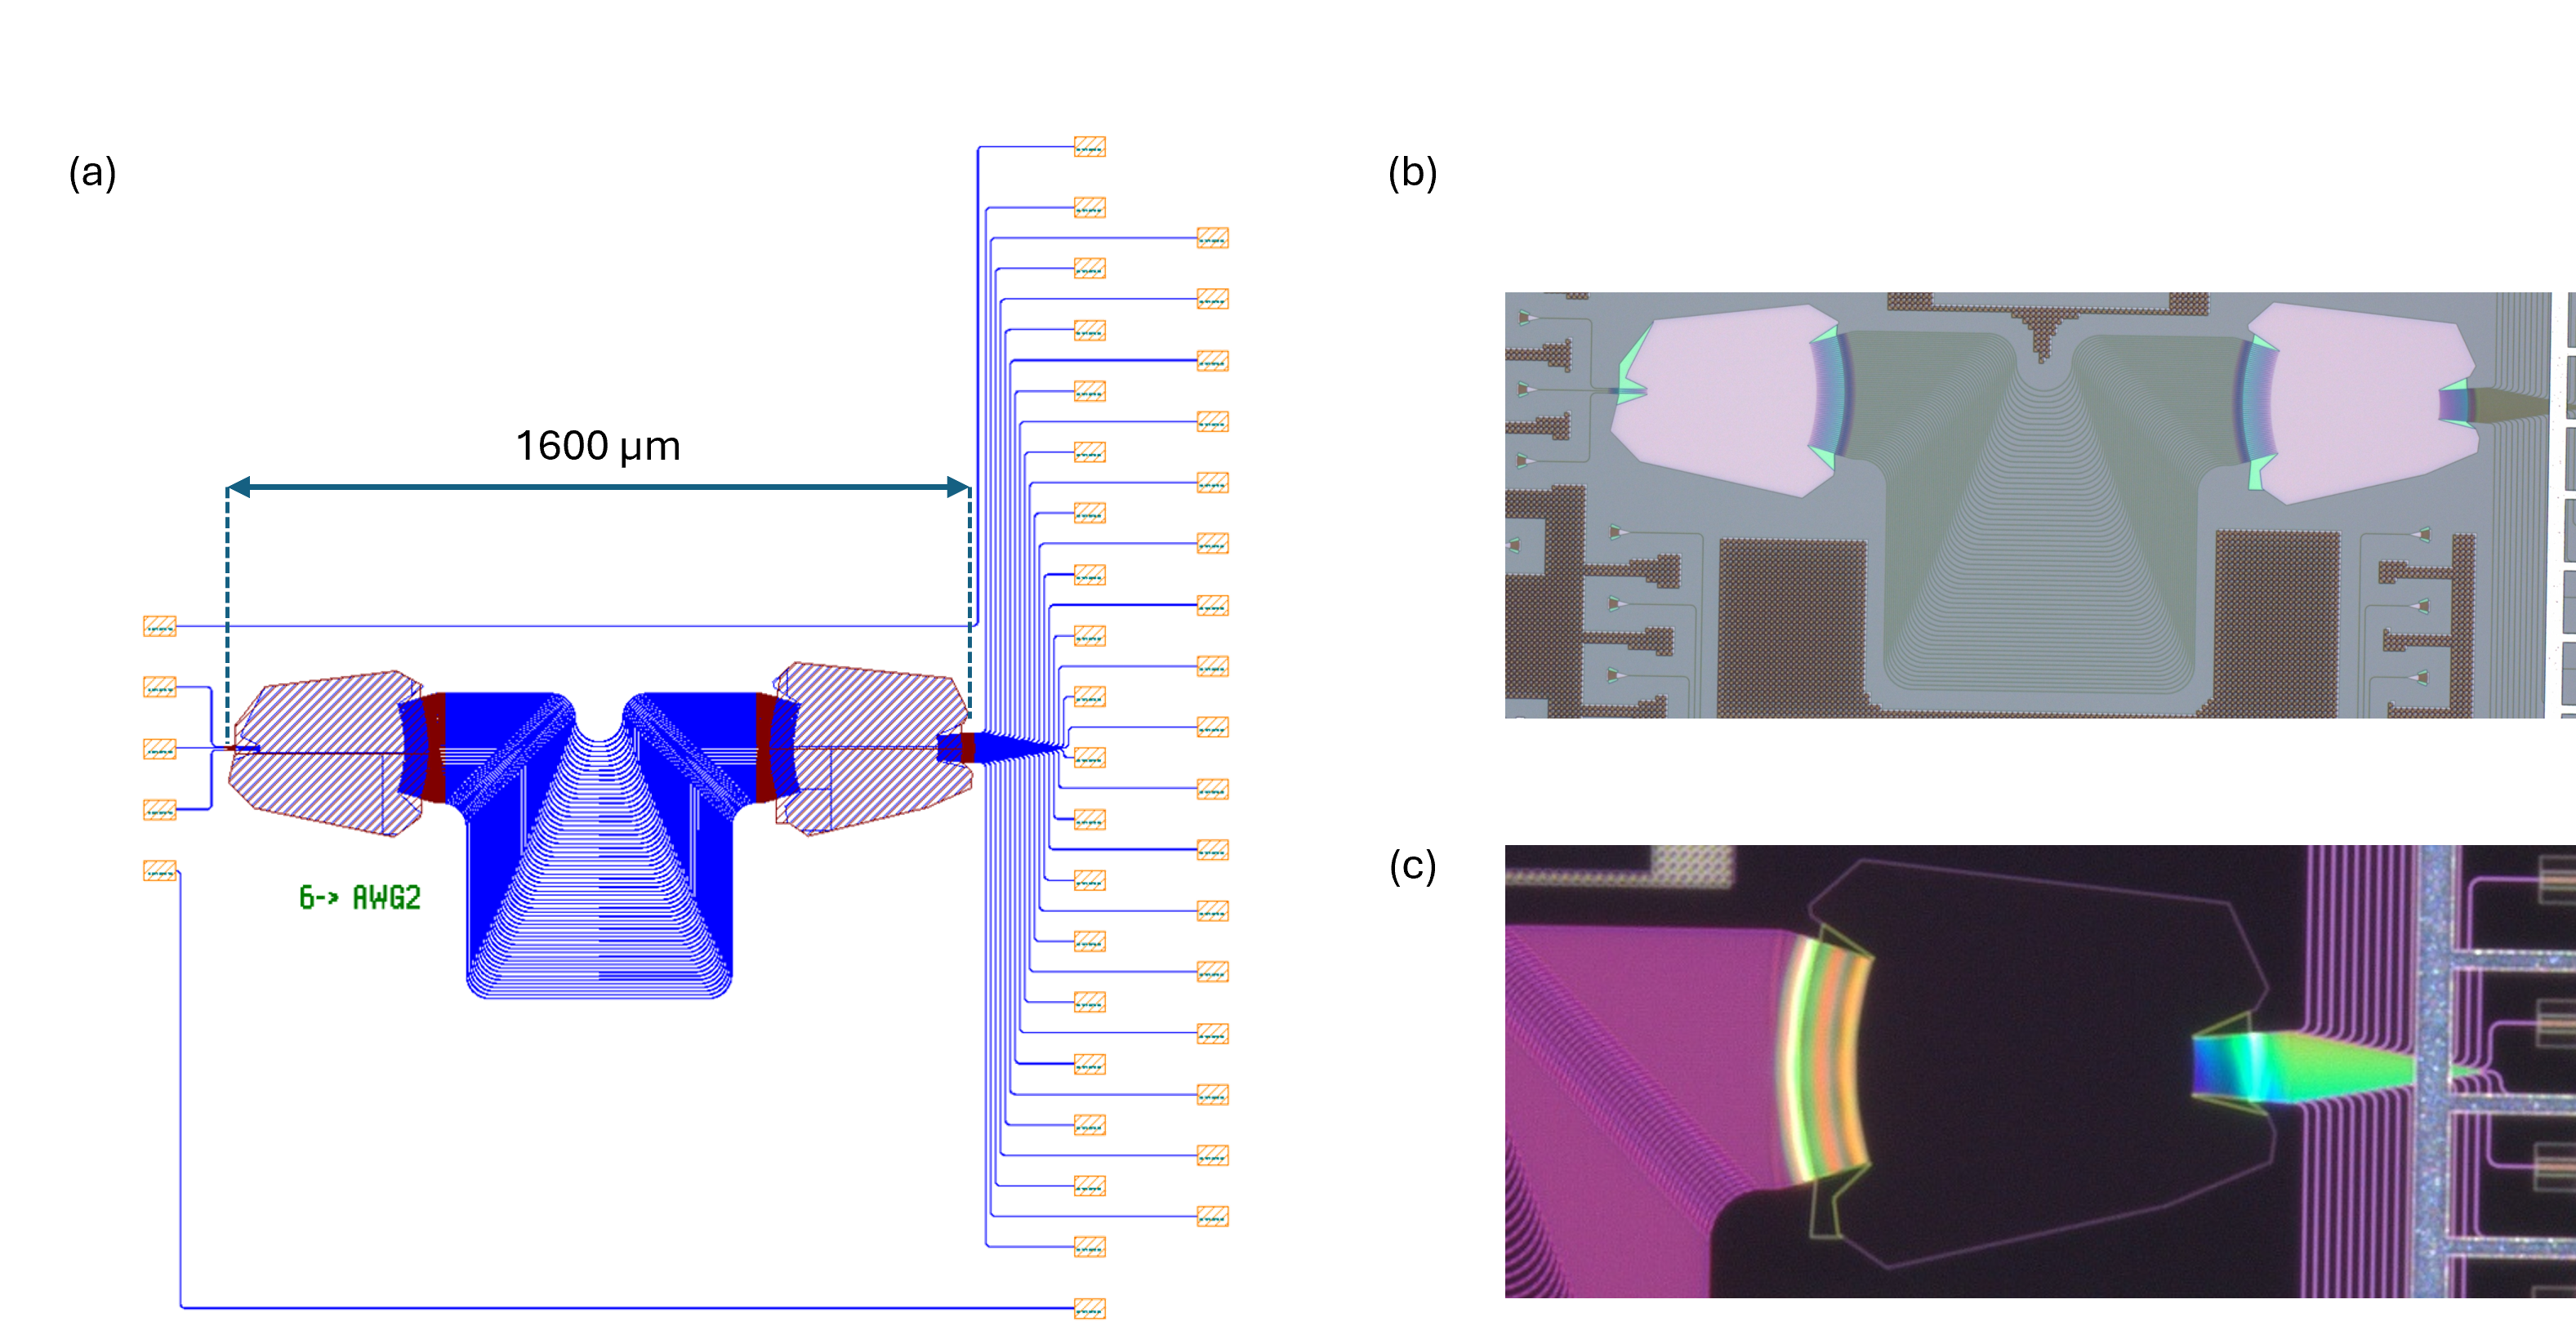
\includegraphics[width=\textwidth]{figures/ch4-awg_test_structures.png}
    \caption{Architecture and physical realization of the test AWG. (a) GDS layout of the complete 
    characterization structure, featuring serialized input and output ports. (b) Optical micrograph 
    of the fabricated device. (c) High-magnification inset of the Free Propagation Region, 
    detailing the Rowland slab interface and the starting section of the phased waveguide array 
    that dictates the device's spectral transfer function.}    
    \label{fig:ch4-awg_test_structures}
\end{figure}


\begin{figure}[htbp]
    \centering
    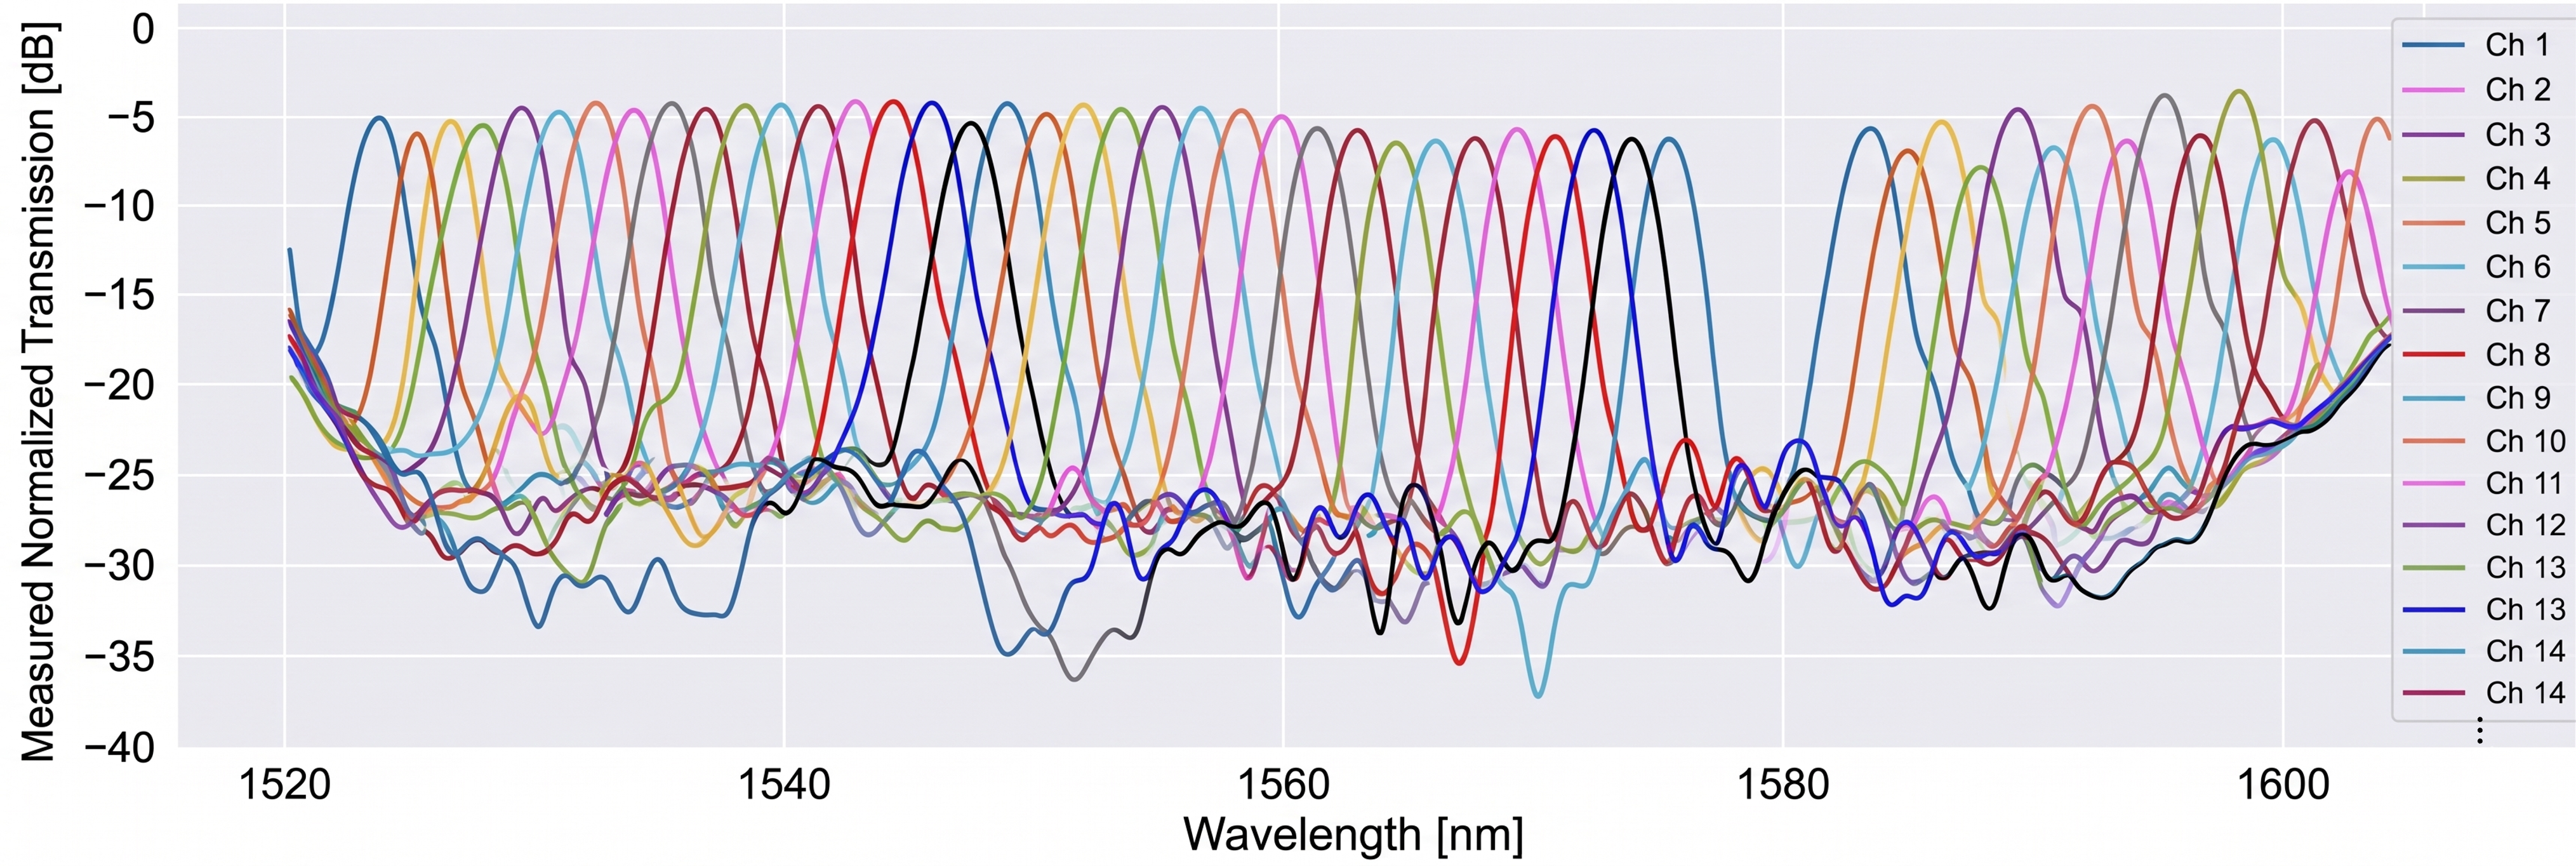
\includegraphics[width=\textwidth]{figures/ch4-awg_measurements.png}
    \caption{Experimental spectral response of the 35-channel test AWG spectrometer.}
    \label{fig:ch4-awg_measured_spectrum}
\end{figure}

\FloatBarrier

Spectral correspondence between the simulated design and the experimental results is illustrated in 
Figure~\ref{fig:ch4-awg_sim_vs_meas}. Measured data for output channel \#0 exhibits high 
morphological fidelity to the simulated response, particularly regarding the main peak width and 
the secondary lobe suppression. However, a noticeable wavelength offset and an expanded FSR are 
present in the fabricated device. Such discrepancies are typically attributed to the sensitivity of 
the phased waveguide array to the effective group index ($n_g$), which slightly differs from the 
nominal values used during the simulation phase due to the over-etching effects identified in 
Chapter 3.

\begin{figure}[htbp]
    \centering
    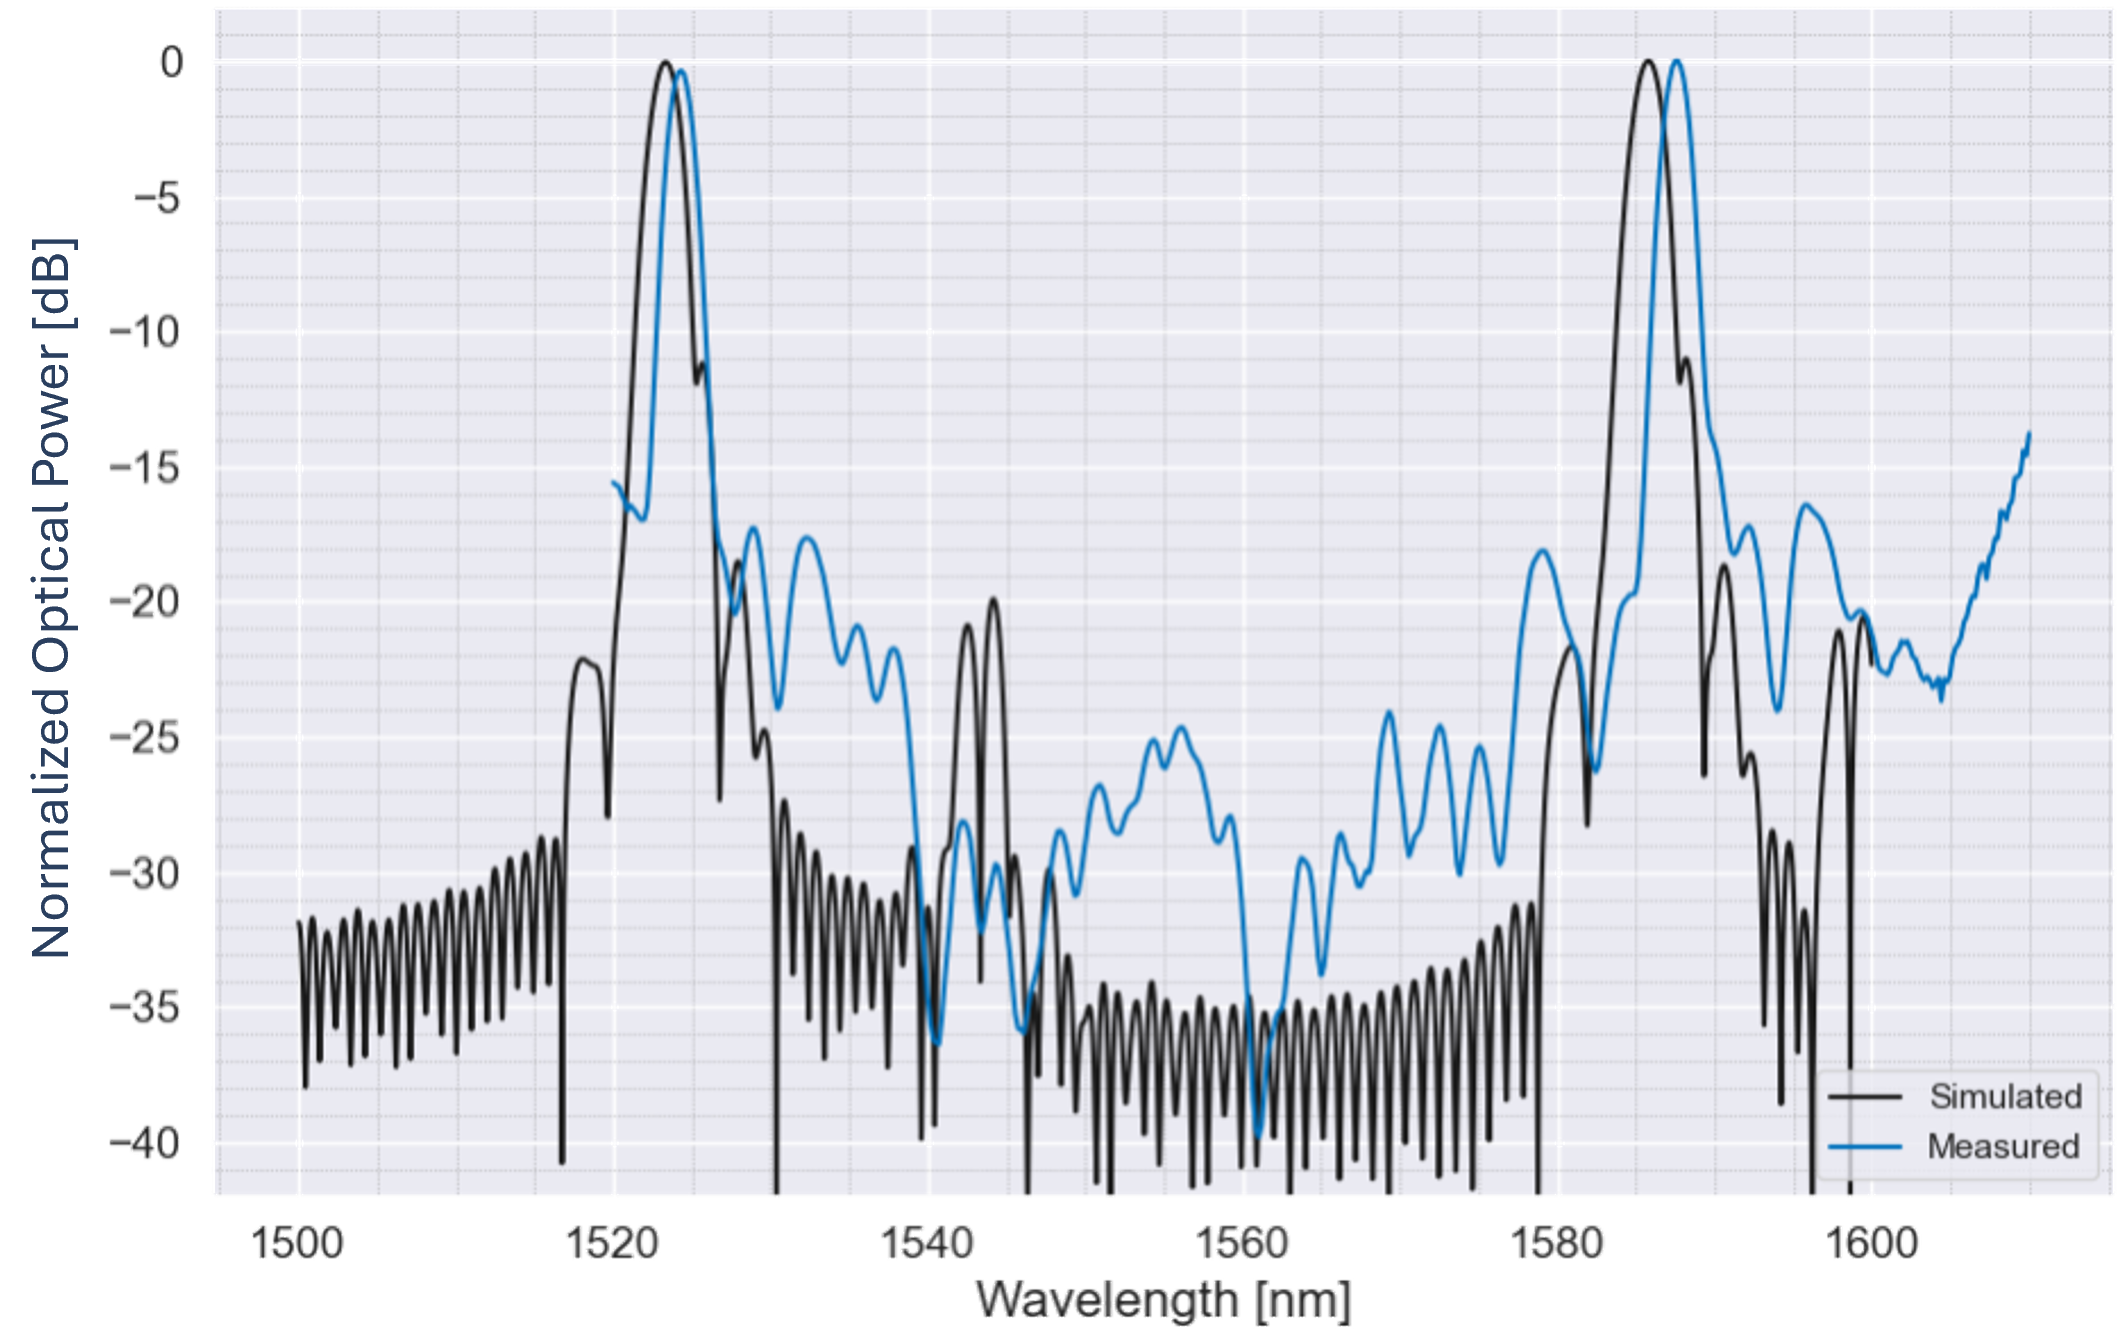
\includegraphics[width=0.8\textwidth]{figures/ch4-awg_sim_meas.png}
    \caption{Comparison between simulated (black) and measured (blue) spectral responses for output 
    port \#0.}
    \label{fig:ch4-awg_sim_vs_meas}
\end{figure}


Beyond the characterization of a single device, the robustness of the AWG design was evaluated 
across five different dies (B7, E6, D5, F3, and G8). This statistical approach is essential to 
quantify the impact of fabrication tolerances on the critical performance metrics of the HPB 
layer. Table \ref{tab:awg_statistical_results} summarizes the measured parameters for these chips, 
compared against the initial design targets.

\begin{table}[htbp]
    \centering
    \caption{Measured performance metrics of the 35-channel AWG across five different dies.}
    \label{tab:awg_statistical_results}
    \resizebox{\textwidth}{!}{%
    \begin{tabular}{lcccccc}
        \hline
        \textbf{Parameter} & \textbf{Target} & \textbf{B7} & \textbf{E6} & 
        \textbf{D5} & \textbf{F3} & \textbf{G8} \\ \hline
        Ch. spacing [nm] & 1.6 & 1.6 $\pm$ 0.1 & 1.59 $\pm$ 0.14 & 1.6 $\pm$ 0.12 & 
        1.6 $\pm$ 0.12 & 1.6 $\pm$ 0.12 \\
        FSR [nm] & 59.2 & 63.40 & 63.46 & 63.47 & 63.53 & 63.41 \\
        IL [dB] & - & 5.14 $\pm$ 0.6 & 5.01 $\pm$ 0.9 & 3.54 $\pm$ 0.9 
        & 3.87 $\pm$ 0.7 & 4.36 $\pm$ 0.7 \\
        Crosstalk [dB] & -10.0 & -12.37 & -10.87 & -9.64 & -9.90 & -11.60 \\ \hline
    \end{tabular}
    }
\end{table}

The experimental data reveals a remarkably consistent channel spacing of 1.6 nm across all samples, 
showing that the angular dispersion of the Rowland geometry is highly resilient to local process 
variations. However, a systematic shift is observed in the FSR, which averages 63.4 nm across the 
dies—approximately 4 nm higher than the design target. This discrepancy likely stems from a slight 
underestimation of the group index ($n_g$) in the silicon waveguides during the simulation phase, 
a common occurrence in SOI photonics due to the high sensitivity of the effective index to the 
final etched waveguide geometry.

Regarding power efficiency, insertion losses demonstrate excellent performance, with values as low 
as 3.54 dB in chip D5. These results are notably superior to the initial conservative estimates, 
validating the use of widened waveguide sections to minimize propagation and scattering losses. The 
intra-channel crosstalk remains well-aligned with the -10 dB requirement, with mean values hovering 
around -11 dB. Although chip D5 and F3 show marginal deviations (-9.64 dB and -9.90 dB 
respectively), the overall isolation remains sufficient to ensure the accuracy of the centroid 
detection algorithms. This high level of reproducibility across the five measured chips confirms 
the reliability of the AWG as a foundational building block for the autonomous transceiver.


\subsection{Dispersion Compensation: Reconfigurable Lattice Filters}
\label{subsec:lattice_design}

The second HPB category addresses the mitigation of physical layer impairments, specifically 
chromatic dispersion. While a hexagonal mesh can implement various filter responses, synthesizing 
the steep and precise phase profiles required for dispersion compensation is more efficiently 
handled by dedicated reconfigurable filters. These filters could be based on lattice 
configurations \cite{djordjevicFullyReconfigurableSilicon2011,binbinguanCMOSCompatibleReconfigurable2014,ibrahimDemonstrationFastreconfigurableSilicon2011},
Ring-Assisted Mach-Zehnder Interferometer (RAMZI) 
\cite{catala-lahozSelfConfiguringProgrammableIntegrated2025}, coupled resonator optical waveguide 
(CROW) \cite{zhuSiliconPhotonicTunable2025}, among others.
Specifically, the type selected as the most appropiate for the programmable dispersion compensation
is a lattice filter \cite{takiguchiDispersionSlopeEqualizer1998}. It consist of cascaded stages of 
Mach-Zehnder Interferometers and delay lines, allowing for the independent control of the magnitude 
and phase response. The synthesis of these filters is geared toward providing a tunable 
inverse-dispersion profile that can compensate for varying lengths of standard single-mode fiber 
(SSMF). 

As we will discuss in Section \ref{sec:inductive_modeling}, the ability to model these lattice 
filters as discrete $2\times2$ blocks is what enables their seamless integration into the larger 
dual-polarization fabric. This modularity allows the smart transceiver to dynamically allocate its 
processing power: using the hexagonal mesh for spatial routing and the lattice filters for 
fine-grained spectral shaping.



\section{Inductive Modeling for Large-Scale Synthesis}
\label{sec:inductive_modeling}

The methodology developed for this kilo-scale architecture addresses the inherent limitations of 
traditional simulation environments when scaling to 1020 PUCs and 332 monitors 
\cite{Santome2026_ECIO}. While previous frameworks relied on piecewise element modeling, the 
approach presented here utilizes an inductive method based on recursive signal flow graphs to 
achieve holistic system-level simulation.

A fundamental advantage of this inductive approach is the systematic concatenation of $2\times2$ 
building blocks. Prior to the development of this tool, the design environment lacked a robust 
mechanism to integrate High-Performance Building Blocks (HPBs)—such as lattice filters—directly 
with the programmable mesh core. By abstracting each component as a four-port network, we can now 
cascade diverse functional stages and predict the global transfer matrix of the dual-polarization 
processor without the exponential computational cost typically associated with large-scale PICs.

This framework also enables a hybrid verification flow. By feeding experimental data from 
individual calibrated blocks back into the signal flow graphs, the simulation accounts for 
real-world fabrication tolerances. This capability was instrumental in synthesizing the complex 
filter responses required for chromatic dispersion compensation, ensuring that the cumulative 
effects of the 1020-cell fabric remained within operational bounds.





% \section{Physical Layout and Electrical Interfacing: Scaling to 1020 PUCs}
% \label{sec:physical_layout}

% Achieving a high-density integration on a $18.7 \times 15.1 \text{ mm}^2$ SOI die demands a 
% meticulous layout strategy to balance optical performance with electrical connectivity. 
% High-resolution definition of the internal waveguide mesh is complemented by an array of flip-chip 
% bonding pads, which serve as the primary electrical interface for the 2040 thermo-optic phase 
% shifters. This packaging-centric design ensures that the photonic core remains accessible and 
% controllable despite the massive number of control signals. Furthermore, the strategic distribution 
% of 332 integrated photodetectors provides a layer of observability that is critical for managing 
% thermal crosstalk and fabrication tolerances in such a large-scale SoC.



